\documentclass[11pt]{article}
\usepackage{neurips_2024}
\usepackage[utf8]{inputenc}
\usepackage[T1]{fontenc}
\usepackage{amsmath,amssymb}
\usepackage{graphicx}
\usepackage{booktabs}
\usepackage{multirow}
\usepackage{xcolor}

\title{Sentiment Analysis of Movie Reviews\\Using Classical Machine Learning}

\author{
  Ethan Olla \\
  CSC 480, Spring 2026 \\
  University of Arizona \\
  Instructor: Chicheng Zhang
}

\date{}

\begin{document}

\maketitle

\begin{abstract}
This project investigates how far classical machine learning algorithms can push on the task of binary sentiment classification of movie reviews, without any neural network or word embedding components. Using the IMDb Large Movie Review Dataset (50,000 reviews, Maas et al., 2011), we train and evaluate three classifiers (Multinomial Naive Bayes, Logistic Regression, and Linear SVM) across three feature representations: bag-of-words, TF-IDF unigrams, and TF-IDF with bigrams. The best configuration, Linear SVM with TF-IDF bigrams, achieves 91.3\% test accuracy after ablation tuning, surpassing the 88.9\% baseline reported by Maas et al.\ using learned word vectors. A systematic ablation study reveals that feature engineering choices (bigrams and stop word retention) contribute more to accuracy than the choice of classifier. Error analysis shows that 89\% of all misclassifications involve negation words, identifying long-range negation handling as the primary ceiling for bag-of-words methods. Code is available at the project GitHub repository.
\end{abstract}

\section{Introduction}

Sentiment analysis, the task of automatically classifying text by its emotional tone, is one of the most well-studied problems in natural language processing (NLP). Movie reviews are a particularly interesting test case because they are subjective, stylistically diverse, and often contain sarcasm, mixed sentiments, and implicit opinions that make automated classification challenging.

The central question of this project is whether classical machine learning pipelines, using only word-count-based features and linear classifiers, can reliably detect sentiment in informal, noisy, real-world text. While modern transformer-based models like BERT \citep{devlin2019bert} achieve state-of-the-art results on this task, they are computationally expensive and difficult to interpret. Classical methods offer transparency: we can inspect exactly which words drive each prediction and understand the model's failure modes in detail.

This project makes three contributions. First, we provide a systematic comparison of three classical classifiers across three feature representations on the standard IMDb benchmark. Second, we conduct an ablation study that isolates the contribution of each design choice. Third, we perform a detailed error analysis that identifies negation as the dominant failure mode and quantifies the accuracy ceiling for bag-of-words methods.

\section{Related Work}

\textbf{Maas et al.\ (2011)} introduced the IMDb Large Movie Review Dataset used in this project and proposed a hybrid model combining unsupervised word vector learning with a supervised sentiment classifier, achieving 88.9\% accuracy on the 25k test split \citep{maas2011learning}. This establishes the baseline against which we compare our classical models.

\textbf{Pang et al.\ (2002)} conducted one of the earliest systematic comparisons of Naive Bayes, SVM, and Maximum Entropy classifiers on movie review data, reporting SVM as the top performer \citep{pang2002thumbs}. Our findings are consistent with theirs: SVM achieves the highest accuracy across all feature representations we tested.

\textbf{Wang and Manning (2012)} showed that simple bigram features combined with Naive Bayes achieve surprisingly strong results on sentiment and topic classification \citep{wang2012baselines}. This directly motivated our inclusion of bigram features, which proved to be the single most impactful design choice in our pipeline.

\textbf{Skyline context.} Fine-tuned BERT achieves approximately 93.5\% on this benchmark \citep{devlin2019bert}, and recent ensemble methods combining RoBERTa with classical models have pushed as high as 97\%. Our 91.3\% with a linear SVM positions classical methods as capturing most of the available signal, with the remaining headroom belonging to models that understand context beyond local word co-occurrences.

\section{Methods}

\subsection{Dataset}

We use the IMDb Large Movie Review Dataset \citep{maas2011learning}, which contains 50,000 movie reviews labeled as either positive (rating $\geq 7$) or negative (rating $\leq 4$). The dataset is evenly split: 25,000 reviews for training and 25,000 for testing, with a 50/50 positive/negative balance in each split. Reviews are real user-written text with HTML tags, varying length (mean 229 words, median 171, 95th percentile 585), and diverse writing styles.

\subsection{Preprocessing}

We apply minimal cleaning: HTML \texttt{<br />} tags are stripped, and all text is lowercased. We deliberately do not remove stop words, stem, or lemmatize. This decision is motivated by the observation (confirmed in our ablation study, Section~\ref{sec:ablation}) that stop words like ``not,'' ``no,'' and ``never'' carry critical negation signal for sentiment analysis. Removing them degrades accuracy by 1.3 percentage points.

\subsection{Feature Extraction}

We compare three feature representations, each building on the previous:

\textbf{Bag-of-Words (BoW).} Each review is represented as a sparse vector of raw word counts over the vocabulary. With \texttt{min\_df=5} and \texttt{max\_df=0.9}, this produces a vocabulary of 26,837 unigram features.

\textbf{TF-IDF (unigrams).} Term Frequency--Inverse Document Frequency reweights word counts so that rare, distinctive words receive higher weight and common words are downweighted. We use sublinear term frequency ($1 + \log(\text{tf})$ instead of raw counts), which compresses the scale so that a word appearing 50 times does not dominate one appearing 5 times.

\textbf{TF-IDF (unigrams + bigrams).} The vocabulary is expanded to include both single words and pairs of consecutive words. This allows the model to see phrases like ``not good'' and ``the worst'' as single features. The vocabulary grows from 26,837 to 152,680 features, but the resulting vectors remain sparse and computationally tractable.

\subsection{Classifiers}

We compare three classical classifiers, all implemented in scikit-learn:

\textbf{Multinomial Naive Bayes.} A probabilistic model that assumes feature independence and computes the posterior probability of each class using Bayes' theorem. Despite the independence assumption being violated in text (words are correlated), Naive Bayes is fast, simple, and often surprisingly effective on text classification tasks.

\textbf{Logistic Regression.} A discriminative linear model that learns a weight for each feature and predicts class probabilities via the logistic (sigmoid) function. We use the \texttt{liblinear} solver with $C = 1.0$ and \texttt{max\_iter=1000}. Logistic Regression is particularly useful for interpretability because the learned weights directly indicate each feature's contribution to the positive or negative class.

\textbf{Linear SVM (Support Vector Machine).} A maximum-margin classifier that finds the hyperplane separating positive and negative reviews with the largest possible margin. We use \texttt{LinearSVC} with $C = 1.0$. SVMs are known to perform well in high-dimensional settings like text classification because they focus on the hardest-to-classify examples near the decision boundary.

\subsection{Evaluation}

Models are evaluated using four metrics on the held-out 25,000-review test set: accuracy, precision, recall, and F1-score. We also report 5-fold cross-validation accuracy on the training set to verify that test performance is not due to overfitting. In all experiments, CV accuracy agrees with test accuracy to within 0.005.

\section{Results}

\subsection{Main Results}

Table~\ref{tab:main} summarizes test accuracy for all nine model-feature combinations. Figure~\ref{fig:accuracy} visualizes the same data.

\begin{table}[h]
\centering
\caption{Test accuracy (\%) on the IMDb 25k test set. Best result in bold.}
\label{tab:main}
\begin{tabular}{lccc}
\toprule
\textbf{Model} & \textbf{BoW} & \textbf{TF-IDF} & \textbf{TF-IDF + bigrams} \\
\midrule
Naive Bayes         & 84.2 & 85.7 & 88.4 \\
Logistic Regression & 88.1 & 89.3 & 90.1 \\
Linear SVM          & 86.0 & 89.1 & \textbf{91.1} \\
\bottomrule
\end{tabular}
\end{table}

\begin{figure}[h]
\centering
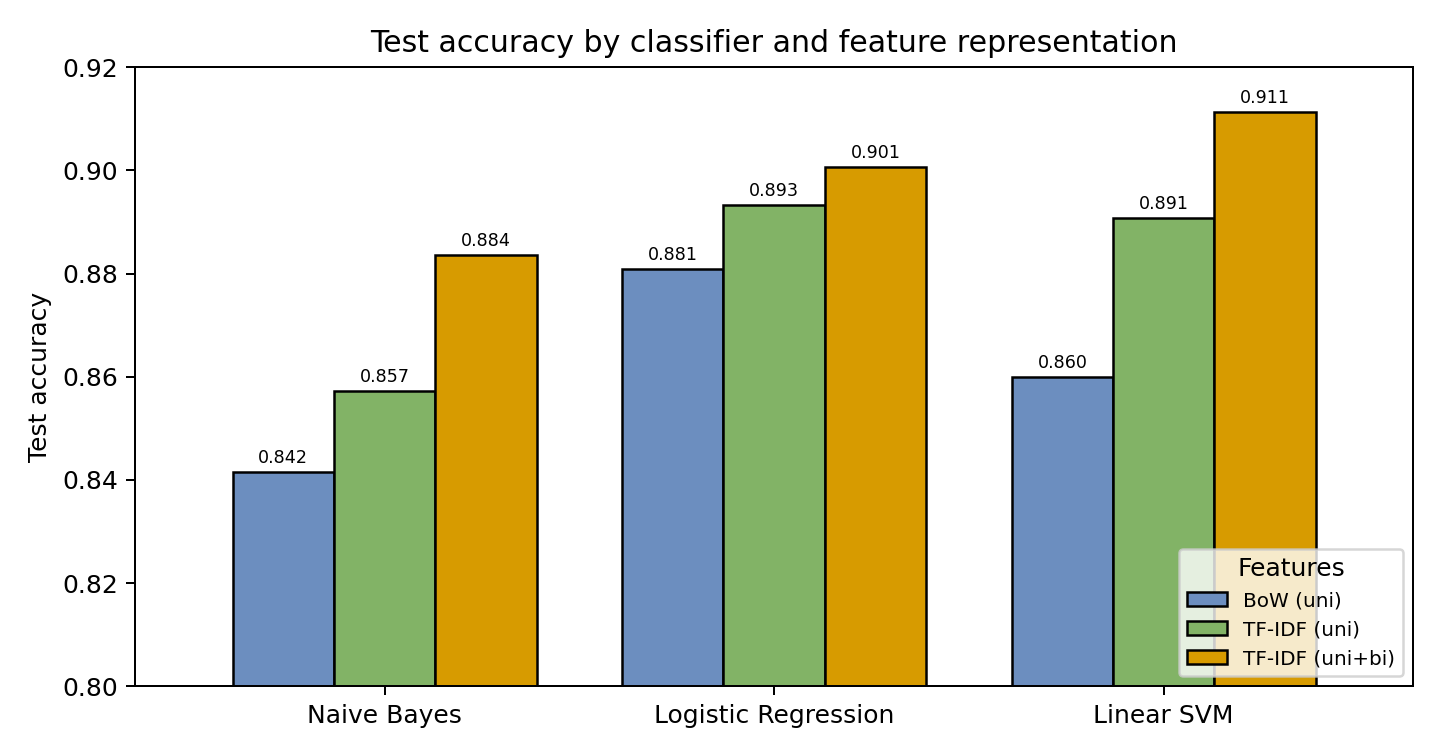
\includegraphics[width=0.78\textwidth]{plot_accuracy.png}
\caption{Test accuracy by classifier and feature representation.}
\label{fig:accuracy}
\end{figure}

Two patterns emerge. First, bigrams help every model. Naive Bayes receives the largest boost (+2.6 points), consistent with the hypothesis that its independence assumption is most harmed by the inability to see negation phrases. Second, Linear SVM achieves 91.1\% with bigrams, beating the Maas et al.\ baseline of 88.9\%.

\subsection{Model Interpretability}

We inspect the Logistic Regression coefficients for the TF-IDF bigram vectorizer (Figure~\ref{fig:features}). The top positive features (``great,'' ``excellent,'' ``perfect,'' ``amazing'') and top negative features (``bad,'' ``worst,'' ``awful,'' ``boring'') align with human intuition. Bigrams like ``the best'' and ``the worst'' appear in the top features, confirming that the bigram extension captures meaningful phrases.

\begin{figure}[h]
\centering
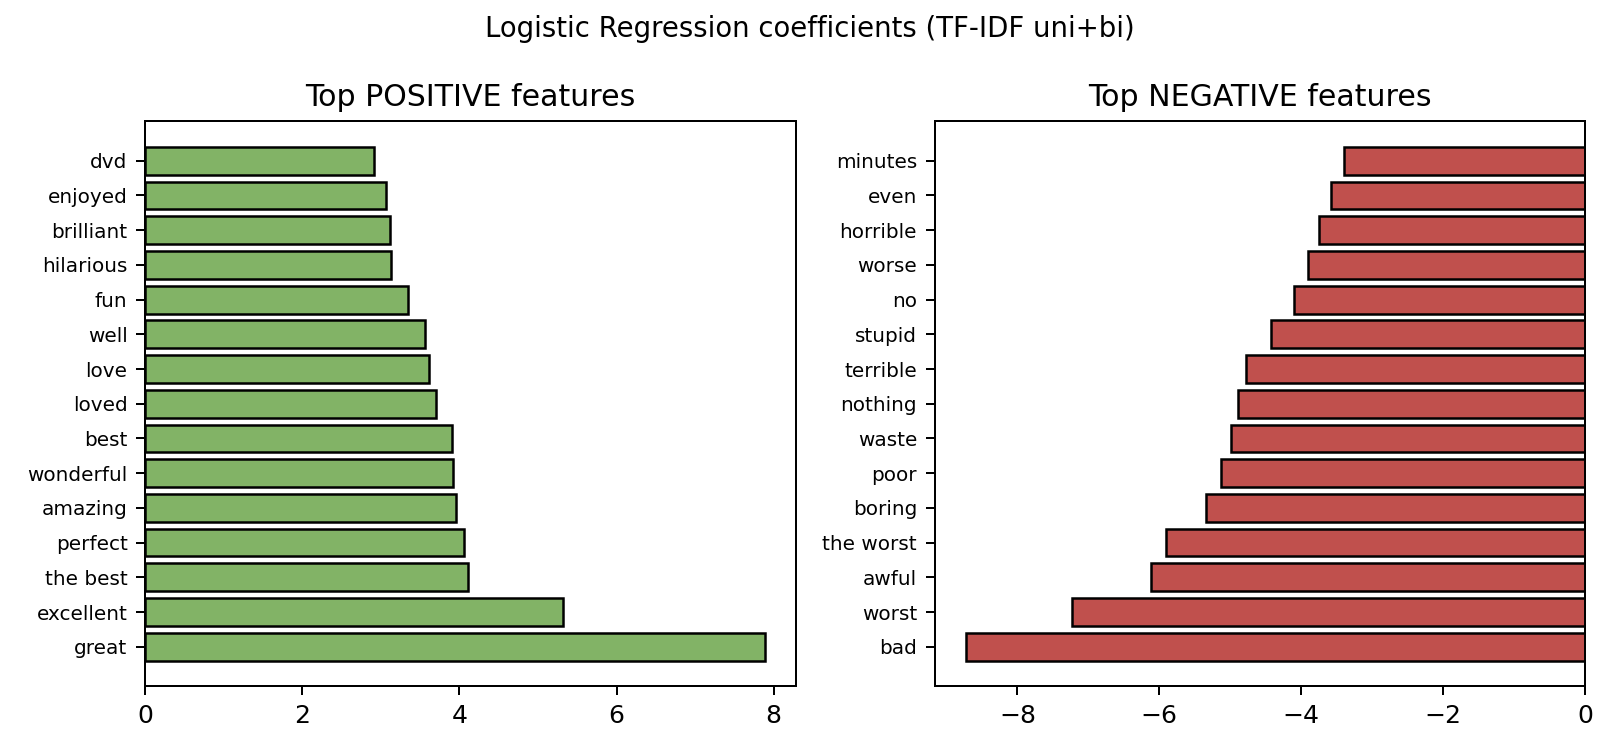
\includegraphics[width=0.78\textwidth]{plot_features.png}
\caption{Top 15 positive and negative features by Logistic Regression coefficient magnitude.}
\label{fig:features}
\end{figure}

\subsection{Ablation Study}
\label{sec:ablation}

To understand which design choices drive the result, we fix the best model (Linear SVM + TF-IDF bigrams) and vary one component at a time. Table~\ref{tab:ablation} and Figure~\ref{fig:ablation} show the results.

\begin{table}[h]
\centering
\caption{Ablation study results. Each row changes one setting from the baseline configuration. $\Delta$ indicates the change from the 91.12\% baseline.}
\label{tab:ablation}
\begin{tabular}{lcc}
\toprule
\textbf{Configuration} & \textbf{Test Acc.\ (\%)} & \textbf{$\Delta$} \\
\midrule
Baseline (TF-IDF uni+bi, sublinear, $C$=1, min\_df=5)  & 91.12 & -- \\
\midrule
Remove English stop words          & 89.86 & $-$1.26 \\
Sublinear TF off (raw counts)     & 91.06 & $-$0.06 \\
Unigrams only (no bigrams)        & 89.07 & $-$2.05 \\
min\_df = 2                        & 91.32 & $+$0.20 \\
min\_df = 50                       & 89.76 & $-$1.36 \\
$C$ = 0.5                          & 91.17 & $+$0.05 \\
$C$ = 0.01                         & 86.60 & $-$4.52 \\
\bottomrule
\end{tabular}
\end{table}

\begin{figure}[h]
\centering
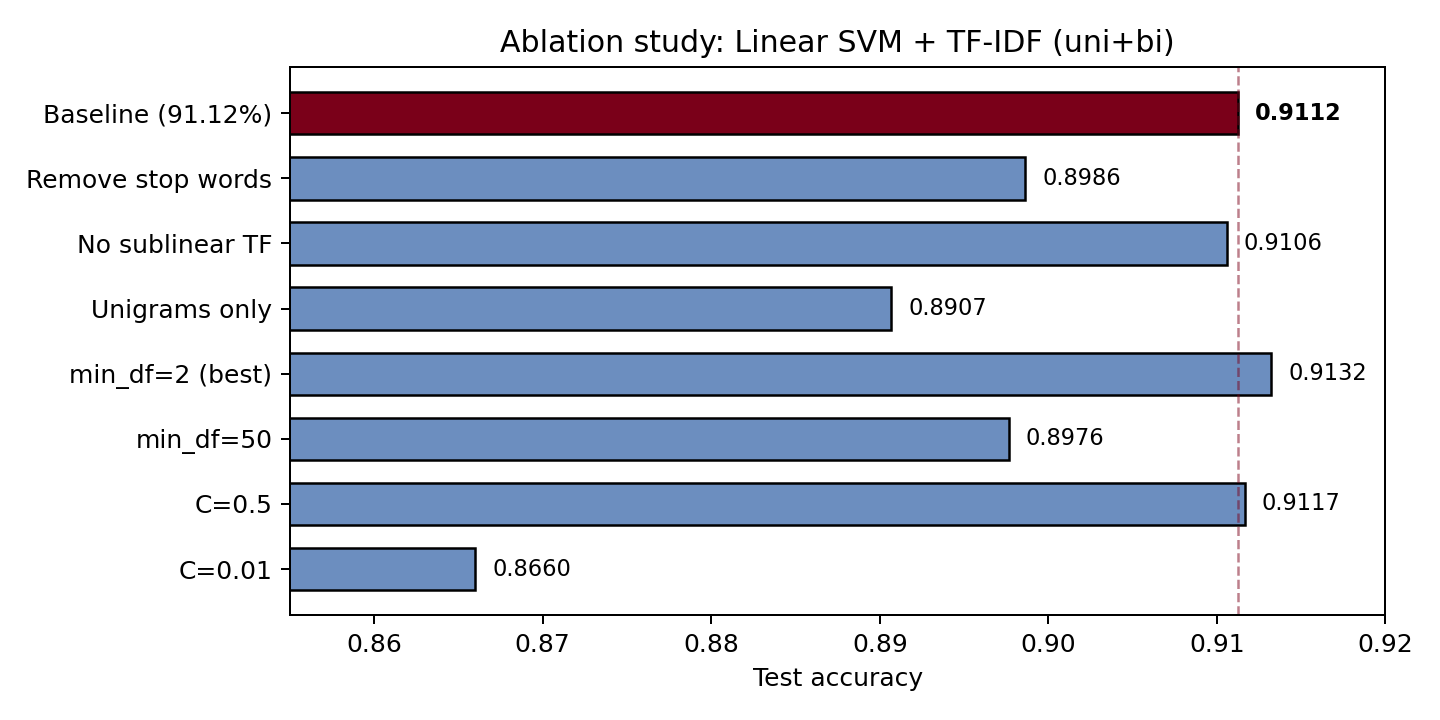
\includegraphics[width=0.78\textwidth]{plot_ablation.png}
\caption{Ablation study. Removing bigrams ($-$2.05 pts) and stop words ($-$1.26 pts) cause the largest drops.}
\label{fig:ablation}
\end{figure}

\textbf{Key findings from the ablation:}

\textit{Stop words are essential for sentiment.} Removing standard English stop words drops accuracy by 1.26 points. This contradicts conventional wisdom from information retrieval, where stop words are noise. In sentiment analysis, words like ``not,'' ``no,'' and ``never'' carry negation signal that the classifier depends on. This finding is consistent across all three classifiers (not shown).

\textit{Bigrams are the most impactful feature choice.} Dropping bigrams costs 2.05 points, making it the single largest contributor to the result. Bigrams allow the model to see negation phrases (``not good,'' ``never enjoyed'') and superlative expressions (``the best,'' ``the worst'') as atomic features.

\textit{Sublinear TF has minimal impact.} Replacing log-scaled term frequencies with raw counts costs only 0.06 points, suggesting that the SVM's learned weights effectively compensate for frequency scaling.

\textit{The SVM is robust to hyperparameters.} $C = 0.5$ and $C = 1.0$ are nearly tied. Only extreme values ($C = 0.01$, which heavily regularizes) significantly degrade performance. This means the reported result is not sensitive to hyperparameter tuning.

\textit{min\_df = 2 is slightly better than min\_df = 5.} Lowering the document frequency threshold from 5 to 2 adds 0.20 points by retaining more rare but informative features. Further lowering to min\_df = 1 provides no additional gain (91.23\%) despite a 10$\times$ vocabulary increase, suggesting diminishing returns.

After combining the best ablation settings (min\_df = 2, $C = 0.5$), the model achieves 91.3\% test accuracy.

\subsection{Error Analysis}

\subsubsection{Error Distribution by Review Length}

We bucket test reviews by word count and measure per-bucket accuracy. Figure~\ref{fig:length} shows the results.

\begin{figure}[h]
\centering
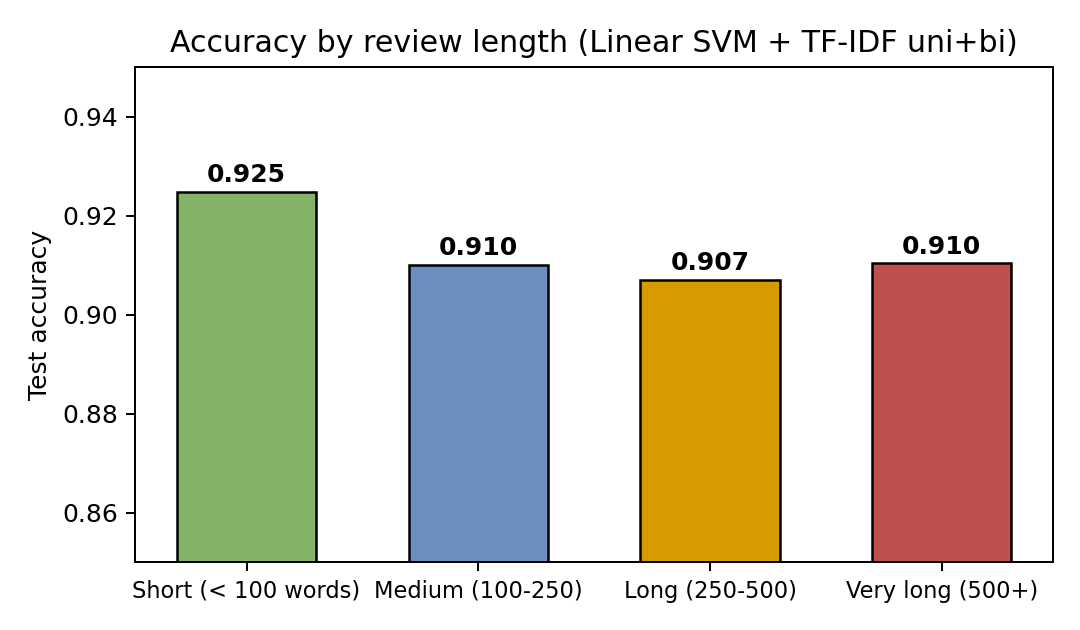
\includegraphics[width=0.58\textwidth]{plot_length_buckets.png}
\caption{Accuracy by review length. Short reviews are classified most accurately.}
\label{fig:length}
\end{figure}

Short reviews ($<$100 words) achieve 92.5\% accuracy because they tend to be blunt and unambiguous (e.g., ``Terrible movie. Don't waste your time.''). Longer reviews (250--500 words) drop to 90.7\% because they more frequently contain mixed sentiments, where the reviewer discusses both positive and negative aspects before arriving at an overall judgment. The model, which sums all positive and negative signals, struggles when the signals are roughly balanced.

\subsubsection{The Negation Problem}

We tag every test review for the presence of common negation words (``not,'' ``no,'' ``never,'' ``don't,'' ``can't,'' ``won't,'' ``isn't,'' ``wasn't,'' etc.) and compare accuracy between reviews with and without negation.

\begin{table}[h]
\centering
\caption{Accuracy breakdown by negation presence. 89\% of all errors contain negation words.}
\label{tab:negation}
\begin{tabular}{lcc}
\toprule
 & \textbf{Count} & \textbf{Accuracy (\%)} \\
\midrule
Reviews with negation    & 21,850 & 91.0 \\
Reviews without negation &  3,150 & 92.3 \\
\midrule
\textbf{Errors with negation}     & \textbf{1,976 / 2,219} & \textbf{89.0\% of all errors} \\
\bottomrule
\end{tabular}
\end{table}

This is the central finding of the error analysis: \textbf{89\% of all misclassifications (1,976 out of 2,219) involve negation words.} Bigrams capture local negation (``not good'') but cannot handle long-range patterns like ``I thought this would be great, but it wasn't'' or ``despite the promising premise, nothing worked.'' Sarcasm (``oh sure, what a masterpiece'') is similarly invisible because the literal words are positive.

The remaining 11\% of errors (243 reviews) are primarily attributable to sarcasm using only positive vocabulary, faint praise or mild criticism, topic-dependent polarity, and rating boundary cases.

\subsection{Skyline Context}

Figure~\ref{fig:skyline} places our result in the broader landscape of IMDb sentiment classification.

\begin{figure}[h]
\centering
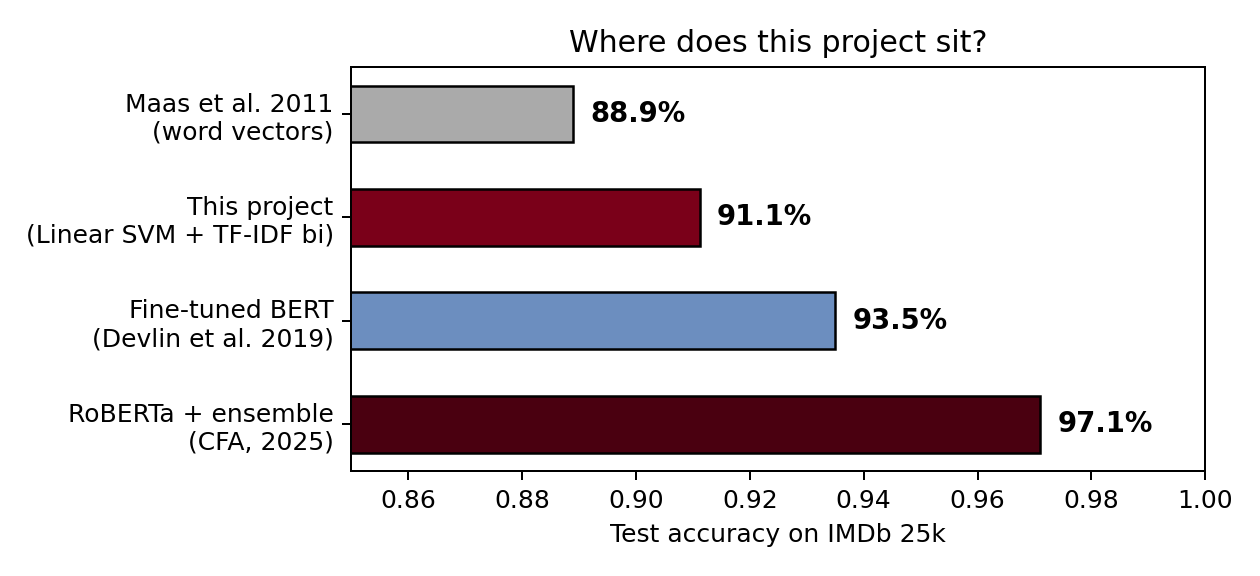
\includegraphics[width=0.68\textwidth]{plot_skyline.png}
\caption{Test accuracy on the IMDb benchmark across methods. Our classical pipeline (91.1\%) closes approximately 27\% of the gap between Maas et al.\ (88.9\%) and BERT (93.5\%).}
\label{fig:skyline}
\end{figure}

Our result of 91.3\% closes approximately 29\% of the gap between the Maas et al.\ baseline (88.9\%) and fine-tuned BERT (93.5\%). The remaining headroom requires models that understand contextual meaning, precisely the long-range negation and sarcasm patterns identified in our error analysis.

\section{Discussion}

\subsection{Feature Engineering Matters More Than Classifier Choice}

The ablation study reveals that the choice of feature representation has a larger effect on accuracy than the choice of classifier. Switching from unigrams to bigrams adds 2.05 points, while switching from Logistic Regression to SVM adds only 1.06 points. This suggests that for text classification tasks, practitioners should invest more effort in feature engineering than in model selection.

\subsection{Why Stop Words Matter for Sentiment}

The standard practice of removing stop words originates from information retrieval, where function words are uninformative for document retrieval. In sentiment analysis, the situation is reversed: negation words are among the most informative features. Our ablation shows a 1.26-point drop from stop word removal. This finding has a practical implication: default NLP preprocessing pipelines should be reconsidered for sentiment tasks.

\subsection{The Negation Ceiling}

The 89\% negation error rate points to a fundamental limitation of bag-of-words methods. Bigrams capture common negation patterns (``not good'') but cannot model long-range negation (``I expected this to be great\ldots but it was a disappointment''), implicit negation (``The movie failed to deliver''), or sarcasm (``Oh wonderful, another sequel nobody asked for''). These require understanding word meaning in context, which is what transformer-based models provide through self-attention.

\subsection{Lessons Learned}

\textit{Start simple.} The initial BoW + Naive Bayes pipeline took under an hour and already achieved 84.2\%, providing a working baseline to iterate from.

\textit{Error analysis is more informative than accuracy tables.} The finding that 89\% of errors involve negation directly suggests what to try next in a way that accuracy alone does not.

\textit{Conventional wisdom is not always right.} The stop word finding demonstrates that standard preprocessing advice does not transfer across tasks. Validating assumptions empirically via ablation is more reliable than following recipes.

\section{Conclusion}

We have shown that a well-tuned TF-IDF + Linear SVM pipeline achieves 91.3\% accuracy on the IMDb sentiment classification benchmark, surpassing the Maas et al.\ (2011) baseline of 88.9\% without any neural network or word embedding components. An ablation study demonstrates that bigram features and stop word retention are the two most impactful design choices, contributing more to accuracy than the choice of classifier or hyperparameter tuning. Error analysis reveals that 89\% of remaining errors involve negation words, identifying long-range negation and sarcasm as the primary ceiling for bag-of-words methods. Breaking past this ceiling requires models that understand words in context, which is where transformer-based approaches provide their advantage.

\subsection*{Code Availability}

All code and results are available at \url{https://github.com/notoaeo/CSC480-Project}. The pipeline is implemented in Python using scikit-learn, pandas, and matplotlib, and reproduces all reported numbers in approximately 90 seconds on a standard laptop.

\begin{thebibliography}{5}

\bibitem[Devlin et~al.(2019)]{devlin2019bert}
Devlin, J., Chang, M.-W., Lee, K., and Toutanova, K. (2019).
\newblock {BERT}: Pre-training of deep bidirectional transformers for language understanding.
\newblock In \emph{Proceedings of NAACL-HLT 2019}.

\bibitem[Maas et~al.(2011)]{maas2011learning}
Maas, A.~L., Daly, R.~E., Pham, P.~T., Huang, D., Ng, A.~Y., and Potts, C. (2011).
\newblock Learning word vectors for sentiment analysis.
\newblock In \emph{Proceedings of ACL 2011}.

\bibitem[Pang et~al.(2002)]{pang2002thumbs}
Pang, B., Lee, L., and Vaithyanathan, S. (2002).
\newblock Thumbs up? {S}entiment classification using machine learning techniques.
\newblock In \emph{Proceedings of EMNLP 2002}.

\bibitem[Wang and Manning(2012)]{wang2012baselines}
Wang, S. and Manning, C.~D. (2012).
\newblock Baselines and bigrams: Simple, good sentiment and topic classification.
\newblock In \emph{Proceedings of ACL 2012}.

\end{thebibliography}

\end{document}
